\chapter{Descrizione generale}

\section{Inquadramento}
La piattaforma è stata progettata con lo scopo di erogare dei servizi tipicamente richiesti in ambito aziendale come la gestione delle
informazioni degli utenti, meccanismi di autenticazioni e autorizzazione, l'invio di
email e la sottoscrizione a servizi generici in versione di prova.
L'erogazione di questi servizi avviene grazie ai seguenti elementi (vedi Figura \ref{fig:Piattaforma}):
\begin{itemize}
    \itemsep0em
    \item \textit{Client}: applicazione \textit{front-end} che permette agli utenti di sfruttare le funzionalità della piattaforma inviando delle richieste alla API e mostrando le risposte.
    \item \textit{API web}: applicazione web server che permette di gestire le richieste del client e fornisce una interfaccia REST per erogare i servizi.
    \item Microservizio Doc: servizio interno che permette di consultare la documentazione degli endpoint della piattaforma.
    \item Microservizio Mailer: servizio interno che gestisce la generazione dei template delle email e l'invio.
    \item \textit{Message Broker}: permette di fare interagire API web e il microservizio Mailer.
    \item \textit{Email System}: sistema esterno utilizzato per l'effettivo invio delle email agli utenti.
    \item Database: permette di gestire i dati in modo permanente.
\end{itemize}

Gli utenti che interagiranno con la piattaforma software possono essere catalogati in utenti semplici e amministratori.
Gli utenti semplici sono da considerare privi di conoscenze tecniche. Gli amministratori che gestiranno l’API, le applicazioni client, il sistema delle mail e il database
sono personale altamente qualificato in grado di effettuare operazioni di monitoraggio, modifica, correzione e aggiornamento dei vari elementi.

\begin{figure}[H]
    \centering
    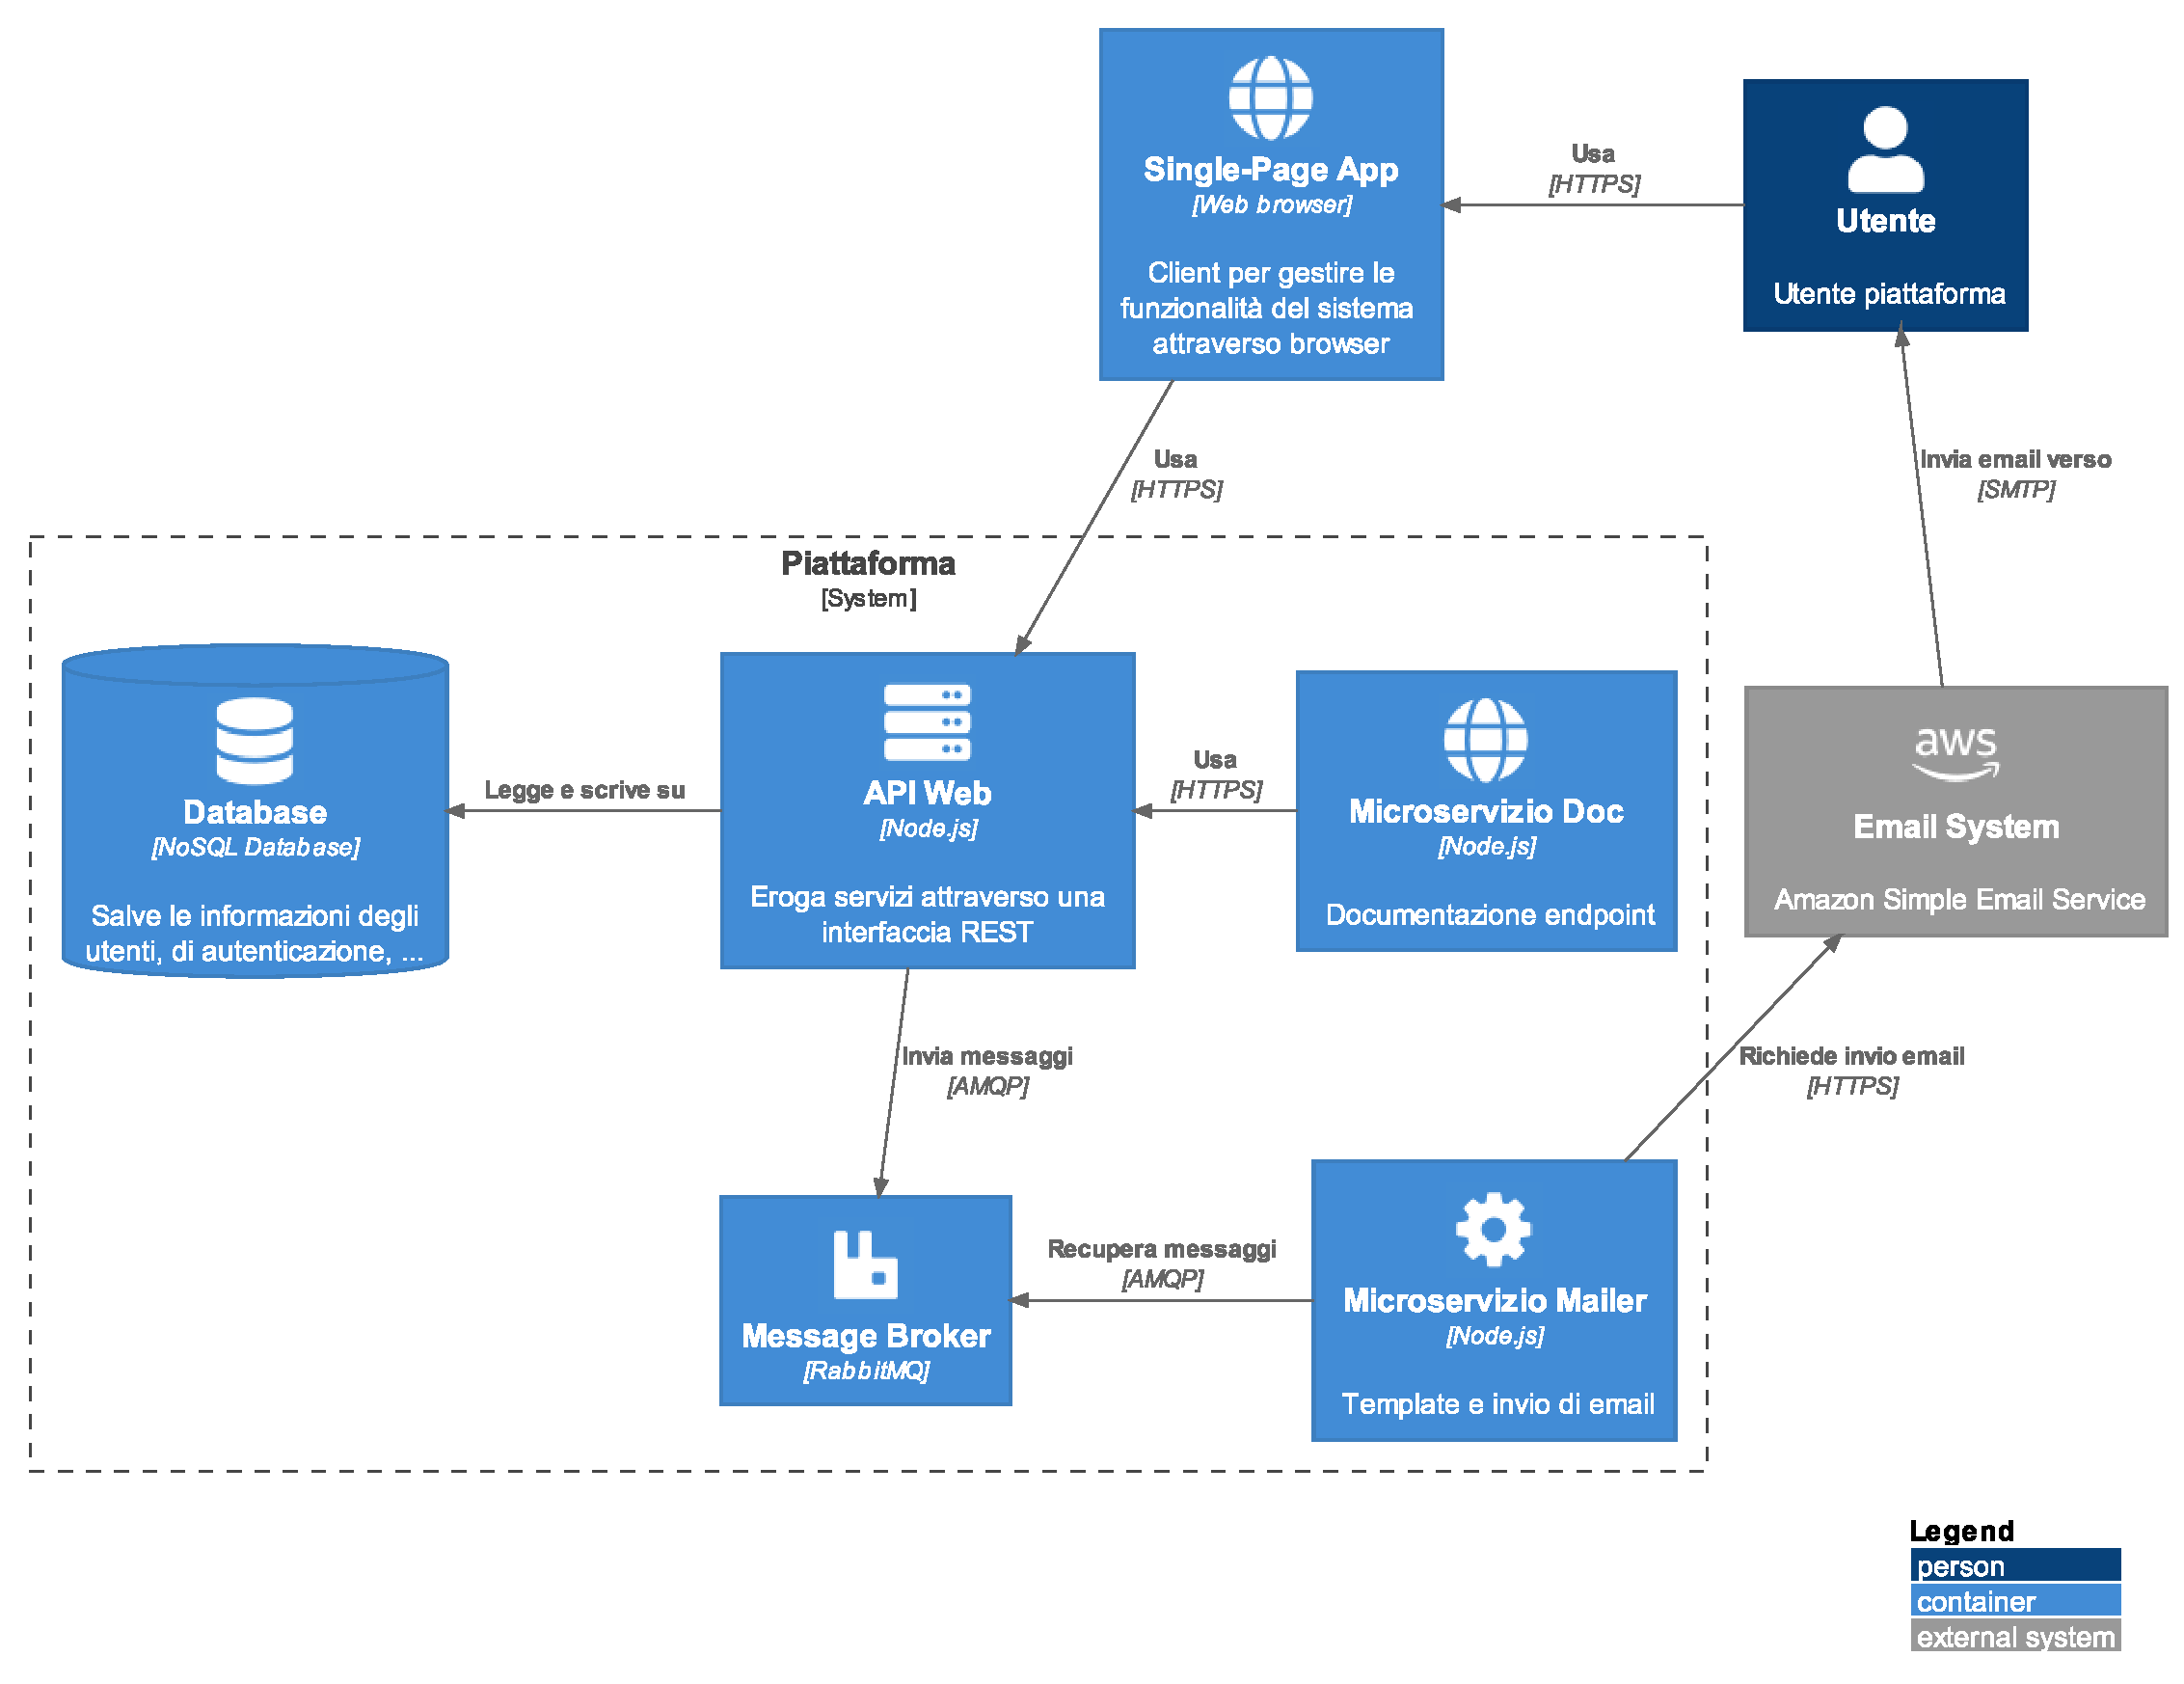
\includegraphics[scale=0.4]{container-diagram-generale.eps}
    \caption{Architettura piattaforma}
    \label{fig:Piattaforma}
\end{figure}

La piattaforma è da considerare come una base su cui costruire e aggiungere i componenti necessari per supportare in maniera efficace il business del
cliente.

\section{Vincoli generali}
\subsection{Requisiti di scalabilità}
La piattaforma deve essere scalabile, ovvero in grado di supportare le operazioni degli utenti
in maniera efficiente.
Pertanto dovrà supportare una possibile transazione a una architettura completamente a microservizi per poter distribuire il traffico e
il carico di lavoro.
Anche le operazioni di supporto al processo di lavoro per la creazione del software deve essere scalabile.
Verranno usate tecnologie, pratiche e metodologie per migliorare l'efficenza delle fasi di sviluppo, verifica e rilascio del prodotto.

\subsection{Requisiti di affidabilità}
La piattaforma deve garantire l'affidabilità dei servizi erogati e mantenere un livello di prestazioni
costante quando viene utilizzata sotto varie condizioni per un dato periodo di tempo.
Deve garantire la presenza di meccanismi di \textit{fault tolerance} per la gestione degli errori, malfunzionamenti o un utilizzo improprio della piattaforma
garantendo la capacità di ripristinare le prestazioni e le informazioni nelle procedure più sensibili.

\subsection{Considerazioni sulla sicurezza}
Il sistema deve garantire la sicurezza degli utenti e l’accesso alle proprie informazioni sensibili.
La privacy degli utenti dovrà essere garantita nel rispetto del Regolamento (UE) 2016/679 GDPR \cite{gdpr}.
Sarà previsto un meccanismo di autenticazione basato su email e password per utenti e amministratori.
Verrà poi implementato un meccanismo di autorizzazione basato sui ruoli e sui permessi di accesso alle singole risorse.
Solo gli amministratori potranno accedere alla API, all’email system e al database.
Per garantire la confidenzialità dei dati scambiati verrà usata una comunicazione sicura tra tutti gli elementi della piattaforma.

\section{Metodologia di lavoro}
La metodologia di lavoro adottata per la realizzazione della piattaforma si ispira alla metodologia Agile e alle pratiche di DevOps.

\subsubsection{Sviluppo}
La metodologia Agile, annunciato ufficialmente nel 2001 attraverso il Manifesto Agile \cite{manifesto},
è un modello di sviluppo finalizzato a rilasciare frequentemente software funzionante e di qualità al cliente.

Questa metodologia prevede che le funzionalità del software vengano rilasciate costantemente
secondo una cadenza molto frequente e non come un singolo prodotto finito.
Il problema della realizzazione del software viene quindi affrontato con l'approccio \textit{divide et impera}:
attraverso una iterazione continua il prodotto software complesso viene suddiviso in sottoprodotti di più semplice comprensione.
I singoli sottoprodotti verranno poi ricomposti come un singolo sistema software.

In questo contesto è inoltre necessario coinvolgere il cliente in maniera costante per renderlo consapevole dell'avanzamento del progetto,
per verificare la comprensione dei requisiti e individuare errori prima di passare alla realizzazione del sottoprodotto successivo.
Questo porta alla realizzazione di cicli in cui interagiscono il team di sviluppo e il cliente: questi si confrontano
per individuare immediatamente problemi nelle funzionalità realizzate e poter così realizzare sin da subito software di qualità.
Questi cicli si ripetono ogni volta che deve essere realizzato un nuovo sottoprodotto. Gli elementi chiave del ciclo sono:
\begin{itemize}
    \itemsep0em
    \item Pianificazione: avviene la raccolta dei requisiti connessi a una funzionalità da implementare
    \item Design: progettazione delle funzionalità
    \item Codifica: vengono implementate le funzionalità incapsulate in componenti
    \item Test: si verifica se ciò che è stato prodotto funziona secondo i requisiti raccolti
    \item Revisione: si raccolgono le opinioni del cliente. In questa fase è possibile individuare errori e verificare la comprensione dei requisiti.
\end{itemize}

\subsubsection{Integrazione e rilascio}
Una volta realizzato il sottoprodotto è necessario metterlo nell'ambiente di produzione per poter così fornire le nuove funzionalità al cliente.
Questa procedura implica l'integrazione dei nuovi artefatti con quelli già prodotti.
La complessità di questa operazione è notevole in quanto bisognerà configurare l'artefatto e l'ambiente per farli cooperare, integrare i nuovi elementi, testare il prodotto risultante
per verificarne il funzionamento e monitorare il nuovo prodotto per individuare problemi durante l'utilizzo.
Queste operazioni solitamente non vengono fatte dal team di sviluppo (\textit{Development Team}) ma dai sistemisti (\textit{Operations team}).
Questi si ritroveranno a dover risolvere dei problemi senza nessuna conoscenza del codice e ciò potrebbe portare a malfunzionamenti del sistema rilasciato al cliente.
Per evitare questa situazione è stato deciso di seguire le pratiche DevOps.

Queste pratiche hanno come scopo l'eliminazione del confine tra i due team andando a considerare questo come un unico gruppo interfunzionale in cui le risorse
siano in grado di acquisire responsabilità riguardanti ogni aspetto ciclo di vita del software. Ciò fornisce a tutti i membri
una conoscenza \textit{end to end} sul sistema.

Le tecniche e i principi DevOps vengono quindi applicati nella metodologia Agile per poter ottimizzare non solo le fasi di sviluppo del software ma
anche le operazioni tipicamente fatte dall'\textit{operations team}.
Questo approccio suddivide il ciclo di sviluppo software nelle fasi di pianificazione, design, codifica, build, test, rilascio, deploy, monitoraggio e operazioni.
Le fasi di pianificazione, design,  codifica e test sono analoghe a quelle della metodologia Agile. La fase di build prevede la compilazione dei componenti realizzati,
la fase di rilascio prevede la pubblicazione del codice sorgente in una repository remota, la fase di deploy consiste nell'installazione del sistema nell'ambiente di produzione
mentre le fasi di monitor e operate consistono nella supervisione dell'ambiente e nella sua configurazione.
Spesso queste fasi vengono supportate con l'uso di tecnologie in grado di automatizzare il passaggio degli artefatti tra una fase e la successiva.

Le pratiche DevOps permettono quindi di ottimizzare l'efficenza del processo di sviluppo del software fornendo degli strumenti utili per favorire la collaborazione fra i vari reparti coinvolti.
Fondendo questa filosofia con la metodologia Agile, che permette di rilasciare software di qualità in un contesto in cui le esigenze sono in continua evoluzione,
è possibile ottenere dei risultati più affidabili e una maggiore efficenza nella gestione complessiva della produzione del software.

\subsubsection{Confronto e valutazioni}
Emerge quindi in modo evidente la contrapposizione con i classici modelli di sviluppo come il modello a cascata.
Questa metodologia ha una struttura rigida composta dalle seguenti fasi: analisi dei requisiti, progettazione, codifica, test, rilascio, manutenzione.
Ogni fase produce degli artefatti che sono necessari per il completamento delle attività nella fase successiva.

Questo implica che tra il contatto con il cliente, in cui avviene la raccolta dei requisiti, e la consegna del prodotto software può passare molto tempo.
Ciò introduce rischi relativi alla realizzazione di un software tecnologicamente obsoleto oppure non in grado di soddisfare le
esigenze del cliente (a causa della mancanza di comunicazione).
Di conseguenza questa metodologia di lavoro non si presta in modo efficiente a quelle organizzazioni dinamiche che non conoscono
a priori i requisiti che vogliono vedere soddisfatti e che necessitano di cambiamenti frequenti nelle operazioni.

Nella realizzazione della piattaforma è stato deciso di seguire la metodologia Agile con l'applicazioni dei principi DevOps e non il modello tradizionale a cascata
erchè si è voluto dare maggiore importanza alla collaborazione fra i team di lavoro, all'ottimizzazione del processo di integrazione e rilascio di aggiornamenti.
Inoltre, visto che il prodotto offerto sarà una personalizzazione realizzata sulla base delle esigenze del cliente
è stata scelta una metodologia di lavoro anche in grado di stimolare la nascita di relazioni costruttive e utili a portare a termine con successo il progetto.


